\documentclass{standalone}
\usepackage{tikz}

\begin{document}
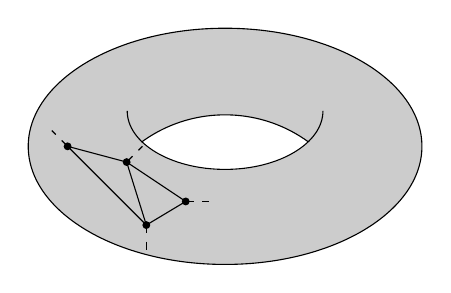
\begin{tikzpicture}
	\filldraw[fill=gray!40] (2,2) ellipse (2.5 and 1.5);
	\begin{scope}
		\clip (2,2.45) ellipse (1.25 and 0.75);
		\filldraw[fill=white] (2,0.6) circle (1.8);
		\draw[thick] (0.75, 2.45) arc[start angle=180, end angle=360, x radius=1.25, y
			radius=0.75];
	\end{scope}

  \fill (0,2) circle (0.05);
  \fill (1,1) circle (0.05);
  \fill (0.75,1.8) circle (0.05);
  \fill (1.5,1.3) circle (0.05);

  \draw (0,2) -- (1,1) -- (1.5,1.3) -- (0.75, 1.8) -- cycle;
  \draw (0.75,1.8) -- (1,1);

  \draw[dashed] (0,2) -- (-0.2, 2.2);
  \draw[dashed] (1,1) -- (1, 0.65);
  \draw[dashed] (0.75,1.8) -- (0.95, 2);
  \draw[dashed] (1.5,1.3) -- (1.8, 1.3);


\end{tikzpicture}
\end{document}

% See if there is such a thing as function declaration in tikz.
